\section{Formáty HDR obsahu} \label{section-formats}

Po vygenerovaní HDR obsahu, sa môže vyžadovať jeho uloženie pre neskoršie úpravy a~spracovanie. Vygenerovaný HDR obsah
s hodnotami v desatinných číslach s pohyblivou rádovou čiarkou, zaberá 96 bitov pre pixel. Na uloženie takého obsahu,
je vhodné obsah komprimovať do jedného zo zavedených formátov, uvedených v tabuľke \ref{table:formats}.
Veľa schém na komprimovanie HDR obsahu je založených na existujúcich štandardoch komprimovania LDR obrázkov.
Cieľom kompresie HDR obrazu je reprezentácia hodnôt s pohyblivou rádovou čiarkou menším počtom bitov.

\begin{table}[h!]
\centering
\begin{tabular}{||c|c|c||} 
  \hline
  Formát & Kódovanie & Bity/pixel \\
  \hline\hline
  \multirow{2}{4em}{HDR} 
  & RGBE & 32 \\ 
  & XYZE & 32 \\
  \hline
  \multirow{3}{4em}{TIFF} 
  & IEEE RGB & 96 \\
  & LogLuv24 & 24 \\
  & LogLuv32 & 32 \\
  \hline
  \multirow{1}{4em}{EXR} 
  & Half RGB & 48 \\
  \hline
\end{tabular}
\caption{Zavedené formáty HDR obsahu \cite{HDRI}}
\label{table:formats}
\end{table}

\subsection*{RGBE}

Formát Radiance HDR (\texttt{.hdr}, \texttt{.pic}), je jeden z prvých formátov pre komprimovanie HDR obsahu. 
Súbor zakódovaný v tomto formáte je zložený z hlavičky so základnými informáciami o parametroch obrázku a komprimovaných 
dát. Pixel uložený vo formáte RGBE má 32 bitov (obr. \ref{fig:rgbe}). Prvých 24 bitov obsahuje jednotlivé farebné kanály v štandardnej
forme hodnôt 0-255 (8 bitov). Posledných 8 bitov je vyhradených pre spoločný exponent. S~ohľadom na to, 
že hodnoty RGB sú vo veľmi podobnom rozsahu, nie je potrebné ukladať exponent zvlášť pre každý farebný kanál.
Exponent je vyjadrený z najjasnejšieho kanálu.

Obmedzením formátu RGBE je, že nemôže reprezentovať vysoko saturované farby v~rámci farebného modelu sRGB. Pri konvertovaní
takýchto farieb sa môže stať, že sa farebné zložky stanú zápornými. V takom prípade RGBE nemôže reprezentovať záporné hodnoty
a niektoré informácie o farbe sa stratia. Riešením tohoto problému je využitie farebného modelu CIE XYZ a kódovanie XYZE. \cite{AHDR}

\begin{figure}[h!]
  \centering
  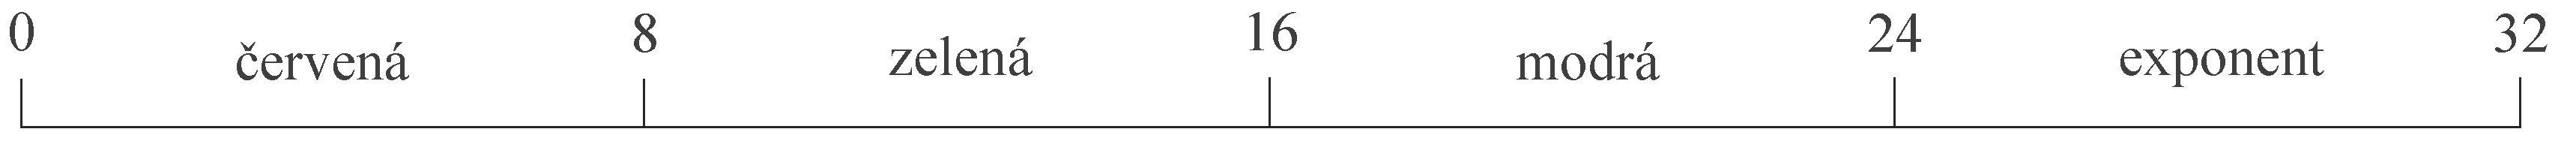
\includegraphics[width=1\textwidth]{figures/storage/rgbe}
  \caption{Formát RGBE, s kódovaním 32 bitov pre pixel}
  \label{fig:rgbe}
\end{figure}

\subsection*{LogLuv}

Kódovanie LogLuv (\texttt{.tif}, \texttt{tiff}), používa na vyjadrenie celého rozsahu jasu a farieb iba celé čísla. Kódovanie
je založené na jave, že ľudské oko nie je rovnako citlivé na všetky úrovne jasu. Ak sa namiesto jasu použije jeho logaritmus,
potom nezáleží na detekovateľných hodnotách prahu, ale konštantné celočíselné hodnoty môžu byť prijateľné pre aproximáciu 
prahu viditeľnosti ľudského oka. \cite{HDRI}

32-bitové kódovanie využíva 16 bitov pre hodnoty jasu a ďalších 16 bitov na reprezentáciu chrominancie (obr. \ref{fig:logluv}).

\begin{figure}[h!]
  \centering
  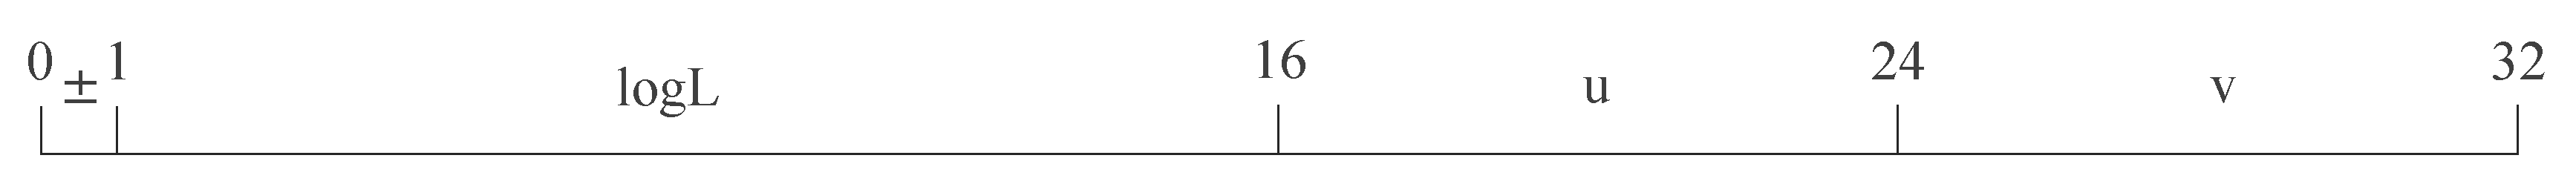
\includegraphics[width=1\textwidth]{figures/storage/logluv}
  \caption{Formát LogLuv, s kódovaním 32 bitov pre pixel}
  \label{fig:logluv}
\end{figure}

\subsection*{OpenEXR}

EXtended Range formát\footnote{\url{http://www.openexr.org}} (\texttt{.exr}) implementovaný v C++ je od roku 2002 dostupný ako open source.
Odvtedy sa stal štandardom pre mnoho aplikácií s HDR obsahom a neustále sa rozvíja aj vo filmovom priemysle. Hodnoty pixelov ukladá
ako 16 alebo 32-bitové číslo s pohyblivou rádovou čiarkou alebo 32-bitové celé číslo. Základná verzia, ktorá využíva 16~bitov
pre farebný kanál, obsahuje 1 znamienkový bit, 5 bitov pre exponent a 10 bitov pre mantisu (obr. \ref{fig:exr}). Formát podporuje
bezstrátovú kompresiu a rozšíriteľnosť knižnice o vlastnú funkcionalitu. \cite{HDRI}

\begin{figure}[h!]
  \centering
  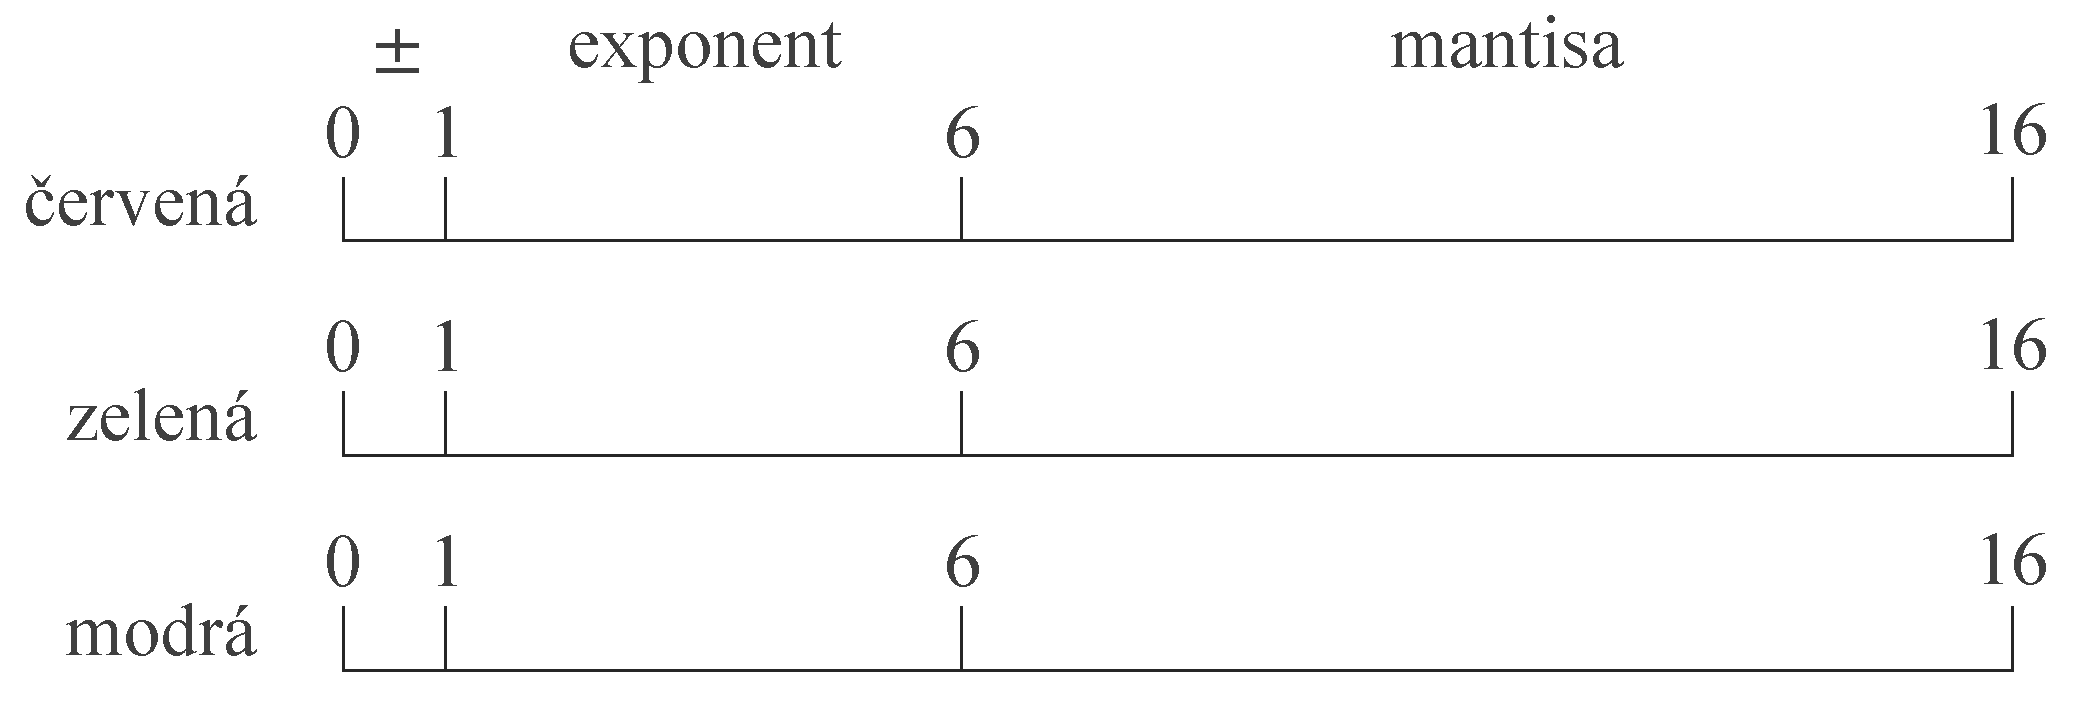
\includegraphics[width=0.6\textwidth]{figures/storage/exr}
  \caption{Formát OpenEXR, s kódovaním 48 bitov pre pixel}
  \label{fig:exr}
\end{figure}